\documentclass[journal]{IEEEtran}

\usepackage{amsmath}
\usepackage{amssymb}
\usepackage{booktabs}
\usepackage{graphicx}
\usepackage{url}
\usepackage{cite}
\usepackage{xcolor}

\begin{document}

\title{Predictable Naming and Malware Sophistication in Software Supply Chain Attacks: A Null Result After Correcting for Taxonomy Coverage and Observational Non-Independence}

\author{%
\begin{tabular}{@{}c@{\hspace{3em}}c@{}}
Tahsin Tajwar Tanni & Nafiz Khan\\[0.3em]
{\small BRAC University} & {\small BRAC University}\\
{\small\texttt{tahsintajwartanni@g.bracu.ac.bd}} & {\small\texttt{nafiz.khan1@g.bracu.ac.bd}}
\end{tabular}%
}

\maketitle

\begin{abstract}
Large language models are known to hallucinate non existent software package names, creating an opportunity for an adversary to pre register the hallucinated name and ship malicious code under it, a pattern termed slopsquatting. A reasonable extension of this threat model is that package names predictable enough for a language model to hallucinate, characterized by compound or trend suffix naming grammar, might correlate with the sophistication of the payload an attacker is willing to invest in, since a low effort naming strategy could plausibly pair with a low effort payload. We test this hypothesis empirically against 401 confirmed malicious package incidents drawn from the GitHub Security Advisory database and the Open Source Vulnerabilities database, spanning the PyPI and npm ecosystems. In the course of this work we identify and correct two methodological failures that materially altered our conclusions. First, a malware payload sophistication taxonomy whose regular expression patterns were derived exclusively from PyPI language produced a near zero detection rate on npm incidents, a coverage gap undetectable from aggregate statistics alone and discovered only through ecosystem stratified cross tabulation. Second, a substantial fraction of npm incident records were found to be non independent observations of the same underlying campaign, reported multiple times across GHSA, OSV, and third party scanner sources, or spread across several squatted package names sharing one payload; treating these as independent observations inflated one stratum's odds ratio to a value as large as 178. After correcting both issues and collapsing the corpus to 142 independent campaign level observations, we find no statistically significant association between naming predictability and malware sophistication, pooled (odds ratio 0.85, p = 0.70) or after Cochran Mantel Haenszel adjustment for ecosystem (common odds ratio 0.93, p = 0.85). We report this null result together with the methodological corrections that produced it, since the corrections themselves, in particular the discovery pattern used to surface each bug, generalize to other security text mining pipelines built on multi source advisory corpora.
\end{abstract}

\begin{IEEEkeywords}
software supply chain security, package hallucination, slopsquatting, malware taxonomy, construct validity, Cochran Mantel Haenszel test, observational independence
\end{IEEEkeywords}

\section{Introduction}

Code generating large language models frequently recommend software packages that do not exist in the target registry, a phenomenon termed package hallucination \cite{spracklen2024}. Because the same hallucinated name tends to recur across prompts and across models, an adversary can pre register the hallucinated name on a public package index and populate it with malicious code, a technique the community has named slopsquatting. The attack class has since been extended beyond package registries to code repositories and to agent skill files consumed by autonomous coding assistants, where hallucination rates as high as 85 percent for repository cloning prompts and 100 percent for skill installation prompts have been demonstrated against production systems \cite{spira2026}.

A natural follow on question, and the one this paper investigates, concerns the attacker's side of the exchange once a squatted name has been claimed. If an attacker chooses a highly predictable name, one following a compound or trend suffix naming grammar of the kind a language model is prone to generate, does that choice correlate with how much engineering effort the attacker subsequently invests in the payload itself. A plausible hypothesis, motivated by cost minimizing attacker models from the vulnerability exploitation literature \cite{allodi2021}, is that low effort naming strategies pair with low effort payloads, since both choices are consistent with an attacker who is work averse across the entire attack, not only in the exploit development stage that the original work averse attacker model addressed.

We test this hypothesis against a corpus of 401 confirmed malicious package incidents collected from the GitHub Security Advisory (GHSA) database and the Open Source Vulnerabilities (OSV) database, covering the PyPI and npm ecosystems. Over the course of the analysis we encountered and corrected two distinct methodological failures, each of which we report in full because the discovery process, not only the final numeric correction, is reusable guidance for similar security text mining pipelines.

The first failure was a construct coverage gap. Our malware payload sophistication taxonomy, itself a correction of an earlier attempt that mistakenly targeted an agent directed prompt injection construct the corpus does not contain (Section \ref{sec:construct}), was built from regular expression patterns derived entirely from PyPI language examples. This produced a flat zero percent malware detection rate on the npm stratum across four independent executions of the pipeline before the gap was diagnosed, since the problem is invisible in pooled statistics and only becomes visible once the analyst stratifies by ecosystem and inspects raw text.

The second failure was a violation of observational independence. GHSA, OSV, and third party scanning services such as Amazon Inspector frequently report the identical underlying incident multiple times under distinct advisory identifiers, and a single campaign frequently squats several distinct package names sharing one payload and one description. Treating each advisory record as an independent observation, as the unmodified pipeline did, inflated the npm stratum's odds ratio to an implausible 178 on a two by two table with single digit cell counts, a result that a Haldane Anscombe correction confirmed was not a small sample artifact alone but reflected genuine double counting.

After correcting both issues and collapsing the corpus to independent campaign level units, we find no statistically significant association between naming predictability and malware sophistication in either ecosystem, pooled, or after adjustment for ecosystem via the Cochran Mantel Haenszel procedure. We present this as a genuine, if currently underpowered, null result, together with the two corrections that produced it.

The remainder of this paper is organized as follows. Section \ref{sec:related} situates the work against the package hallucination and agent directed injection literatures. Section \ref{sec:methods} describes data collection, the construct validity correction that preceded this paper's main contribution, the naming grammar classifier, and the statistical design, including both corrections in detail. Section \ref{sec:results} reports the corrected campaign level results. Section \ref{sec:discussion} discusses the findings and their statistical power. Section \ref{sec:limitations} states threats to validity. Section \ref{sec:future} outlines the prioritized path to a properly powered follow up study, and Section \ref{sec:conclusion} concludes.

\section{Related Work}
\label{sec:related}

Package hallucination was first systematically measured by Spracklen et al. \cite{spracklen2024}, who generated 576{,}000 code samples across sixteen popular code generating models and two programming languages, finding that hallucination is a persistent and systemic property of code generating language models rather than an artifact of any single model or prompting strategy, and proposing mitigation strategies including retrieval augmented generation and self detection that measurably reduce, without eliminating, the hallucination rate.

A concurrent and rapidly developing line of work has extended the same underlying mechanism, an adversary pre registering a resource name a language model is likely to hallucinate, beyond package registries. Spira et al. \cite{spira2026} demonstrate an untargeted, pull based indirect prompt injection attack against production coding assistants with integrated terminals, in which a hallucinated repository or agent skill name is pre registered by the attacker and paired with a prompt injection payload that hijacks the assistant once the hallucinated resource is fetched, achieving hallucination rates up to 85 percent for repository cloning prompts and 100 percent for skill installation prompts, and demonstrating remote code execution against several production systems.

This agent directed line of work is mechanistically distinct from the present study. The attack Spira et al. describe relies on text embedded in the squatted resource that is itself designed to manipulate an autonomous agent reading it, an adversarial prompt. The corpus this paper analyzes, GHSA and OSV confirmed malicious package advisories, was found during an early stage of this project (Section \ref{sec:construct}) to contain no such agent directed text; it instead contains third person forensic narration, written by a human security analyst, describing what the malicious code does once installed and executed. The two literatures therefore concern different attack surfaces, hallucinated skill names hosting adversarial prompts that manipulate an agent, versus squatted package names shipping malicious code that executes on install, and the present paper's contribution, the relationship between naming predictability and payload sophistication within conventional package squatting, is not addressed by the agent directed literature.

Hillah et al. \cite{hillah2026} propose a Bayesian calibration layer over existing slopsquat detectors, replacing a binary flag or do not flag decision with a posterior probability derived from an explicit epistemic taxonomy of prior evidence quality. Their approach operates on package registration metadata rather than documentation or advisory text, and does not make a naming grammar correlation claim; it is complementary to, rather than overlapping with, the present analysis.

The theoretical motivation for this paper's original hypothesis, that cheap naming choices might pair with cheap payload choices, draws on the work averse attacker model of Allodi, Massacci, and Williams \cite{allodi2021}, who show empirically, across attack signatures from more than one million real systems, that mass attackers behave as though exploit development carries a large fixed cost, preferentially reusing a small number of vulnerabilities per software version rather than weaponizing every available vulnerability. We note in Section \ref{sec:discussion} that this theoretical anchor is weakened, though not eliminated, by the null result this paper reports; it remains a plausible hypothesized direction for a properly powered follow up study rather than an explanation for an observed effect.

\section{Data and Methods}
\label{sec:methods}

Figure \ref{fig:methodology} summarizes the data collection, labeling, and correction pipeline.

\begin{figure*}[t]
\centering
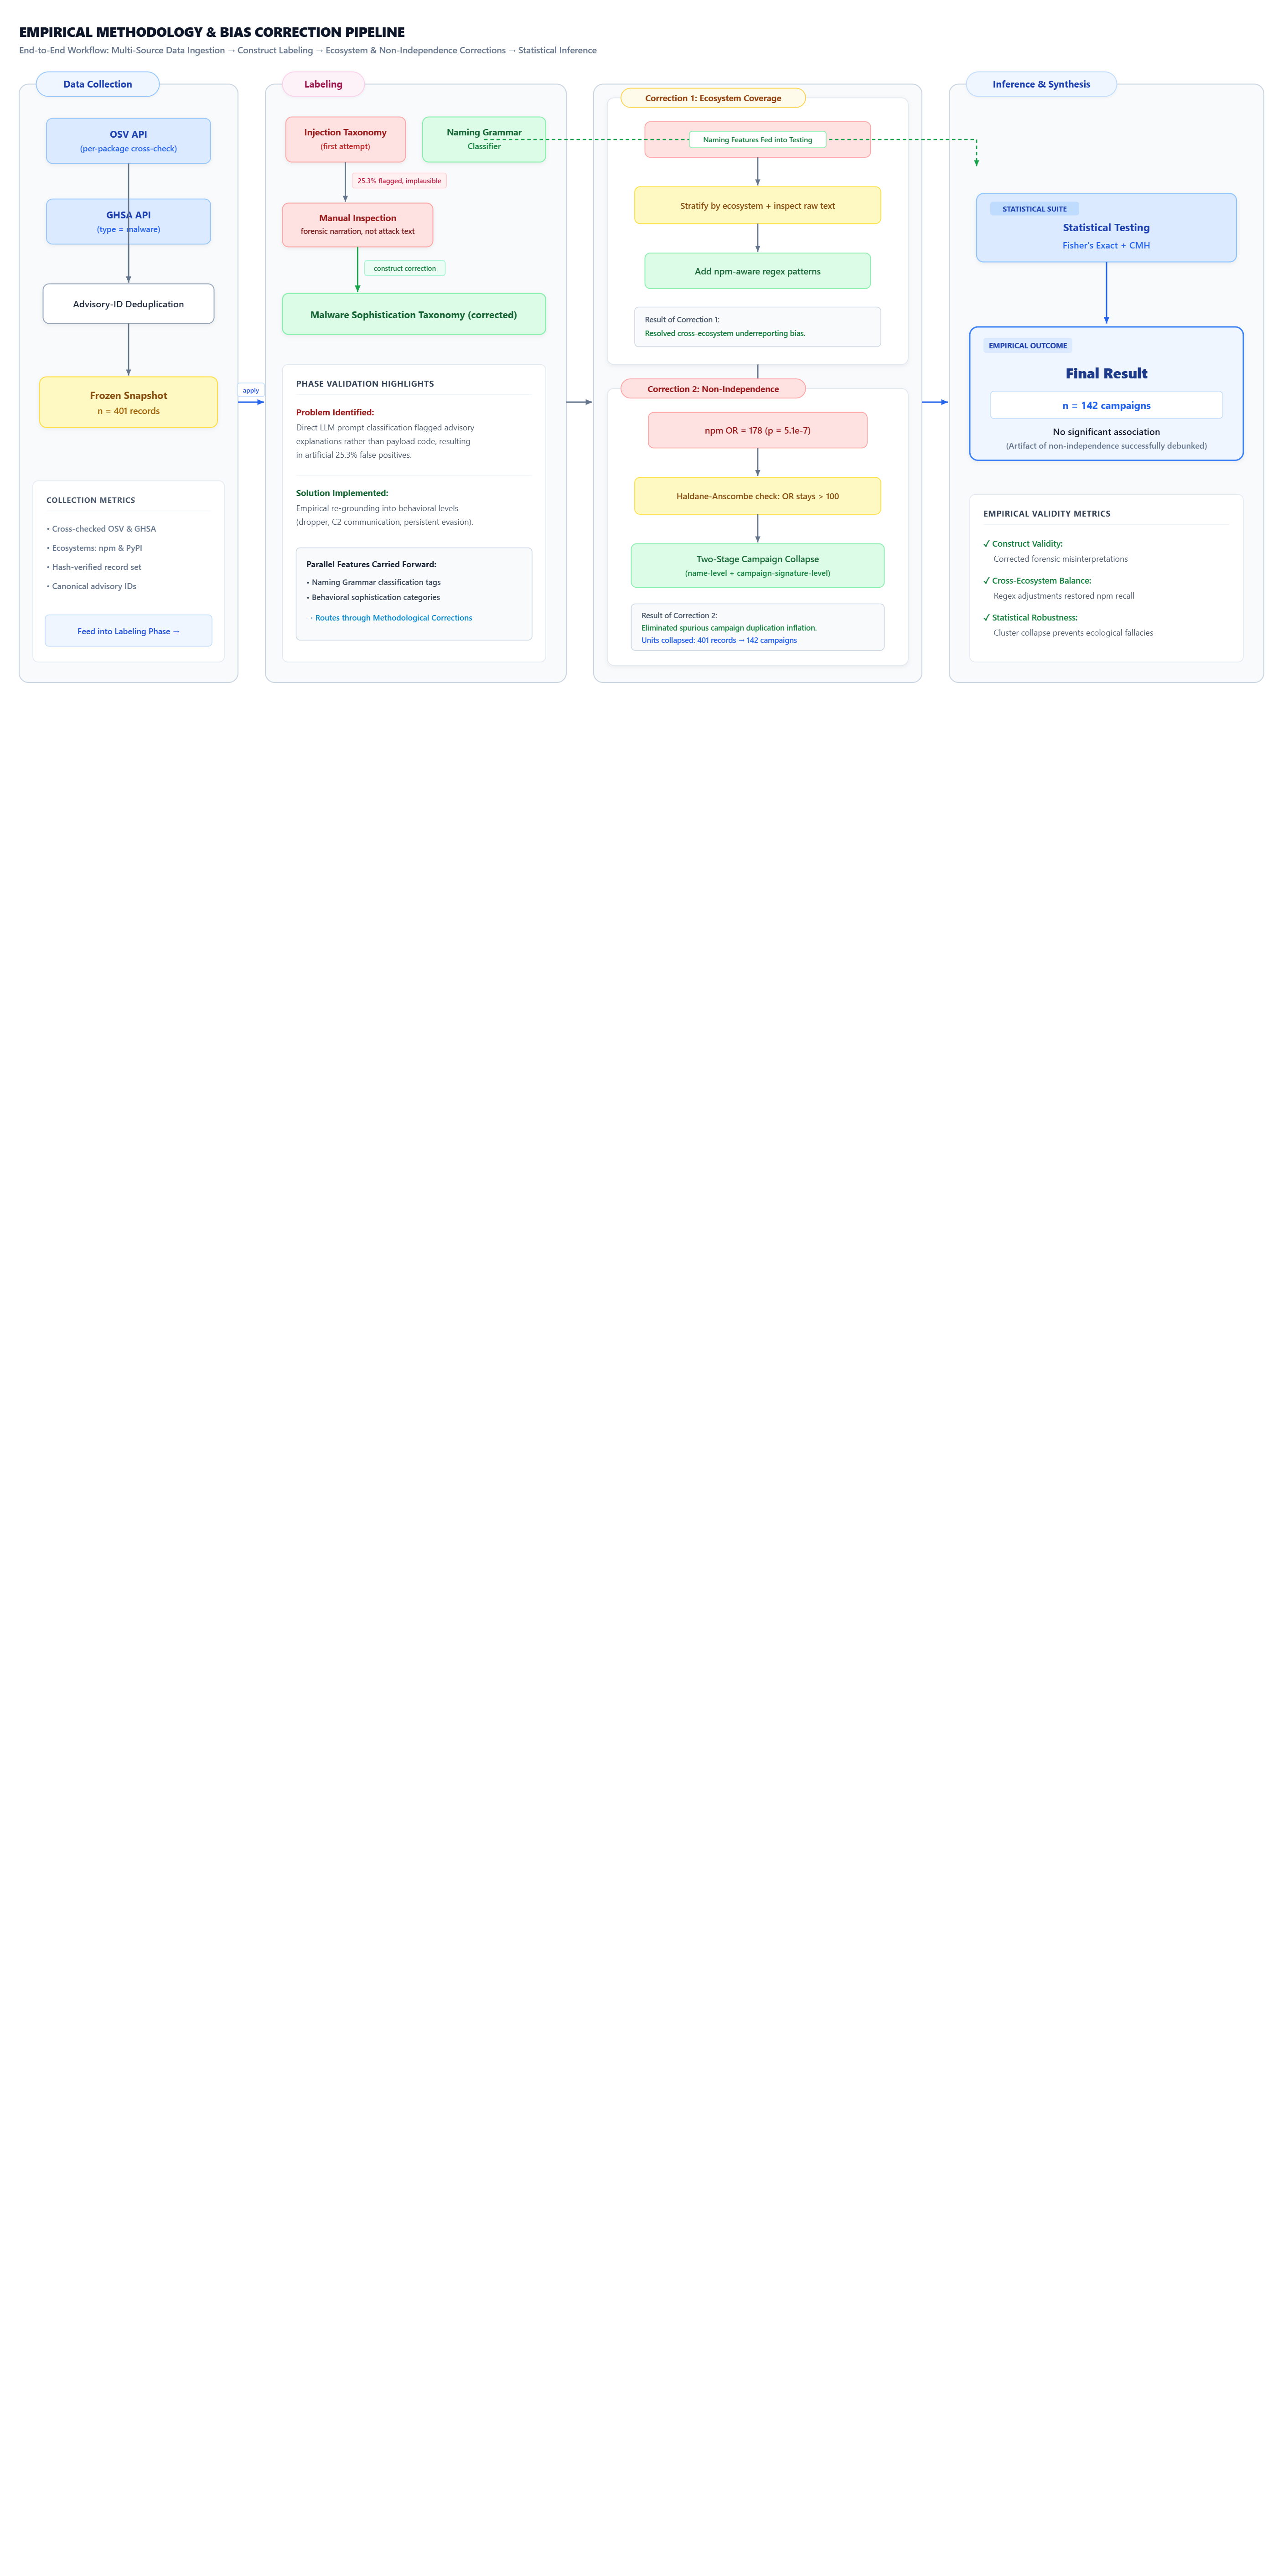
\includegraphics[width=\textwidth,trim=12bp 4108bp 12bp 12bp,clip]{prism-uploads/screen_2.png}
\makeatletter
\long\def\@makecaption#1#2{%
\@IEEEfigurecaptionsepspace
{\normalfont\footnotesize\centering #1.\nobreakspace\nobreakspace #2\par}}
\makeatother
\caption{Overview of the data collection, labeling, and correction pipeline.}
\label{fig:methodology}
\end{figure*}

\subsection{Data Collection}

Confirmed malicious package incidents were collected from two public sources. GitHub Security Advisories were retrieved via the public GHSA API (\texttt{api.github.com/advisories}), filtered to advisory type \texttt{malware} and ecosystems \texttt{pip} and \texttt{npm}. Open Source Vulnerabilities records were retrieved per package, as a cross check and corroboration source, via the OSV query API (\texttt{api.osv.dev/v1/query}), using the package names surfaced by the GHSA pull as the candidate list, since OSV exposes a per package query interface rather than a bulk listing endpoint. Both sources are public and require no authentication at pilot collection volume.

The pipeline deduplicates on the composite key of ecosystem, package name, and advisory identifier, preferring the GHSA record when both sources report an identical advisory identifier for the same package, while retaining distinct advisory identifiers for the same package as separate records, since these may represent genuinely distinct incidents reported through different disclosure channels. As Section \ref{sec:nonindependence} details, this advisory identifier keyed deduplication is correct for its stated purpose but does not catch every form of duplication present in the corpus.

The snapshot analyzed in this paper comprises 401 incident records after this first stage of deduplication, spanning 201 PyPI records and 200 npm records. The snapshot was frozen to a checksummed, versioned file once the corrections described below were validated, specifically to prevent GHSA's status as a live, non static API from introducing further drift into the reported numbers; prior to freezing, successive pulls of the corpus across the project's lifetime returned record counts ranging from 395 to 401, a known and expected source of minor variation in live security advisory data that is immaterial once a single frozen snapshot is adopted for final analysis.

\subsection{Construct Validity: From an Injection Taxonomy to a Malware Sophistication Taxonomy}
\label{sec:construct}

An initial labeling approach targeted a ten category taxonomy of agent directed prompt injection content, under the hypothesis, consistent with this paper's original framing, that package documentation might contain text designed to manipulate an autonomous agent reading it. Applied to the incident corpus, this taxonomy flagged 25.3 percent of records, with every match falling into one of only three categories concerned with execution and resource retrieval instructions, and zero matches in any of the categories specific to agent manipulation, such as direct instruction override or system prompt impersonation.

Manual inspection of the matched text, prompted specifically because this category distribution appeared implausible for a corpus genuinely containing agent directed content, revealed that the matched spans were generic third party scanner verdict language, of the form \textit{Category: MALICIOUS, the campaign has clearly malicious intent, like infostealers}, rather than text embedded in the malicious package intended to manipulate a reader. Further inspection confirmed that GHSA and OSV description fields contain third person forensic narration written by a human security analyst describing the malicious code's behavior, not agent directed documentation text.

This taxonomy was retained in the project's codebase, explicitly scoped for a future corpus genuinely containing agent directed content, such as the agent skill corpora described in Section \ref{sec:related}, but was not applied to the analysis in this paper. A corrected taxonomy targeting malware payload sophistication directly, rather than an agent manipulation construct the data source does not contain, was built instead, with six categories: obfuscated payload execution, hidden install hook, credential or wallet exfiltration, remote backdoor access, remote payload retrieval, and brand impersonation narrative. Each category's regular expression patterns were derived from real examples drawn from the pilot corpus itself, rather than written from first principles before inspecting data, a deliberate methodological correction given that the latter approach caused the first taxonomy's failure. The labeling function's signature accepts only free text, with no package name or naming grammar classification parameter, a structural property enforced by an automated test, since the naming grammar association test reported in Section \ref{sec:results} would be circular if the malware label were computed with knowledge of the package name.

\subsection{Naming Grammar Classification}

Package names are classified as grammar flagged or not using compound and trend suffix pattern matching, ported and extended from an earlier exploratory project's candidate generation logic, repurposed here from generating candidate hallucinated names to classifying observed names. Trend suffix patterns include endings such as \texttt{-turbo} and \texttt{-pro}, chosen to capture naming conventions plausible for a language model to hallucinate. This classification is computed from the package name string alone and does not read the malware label, preserving the independence required for the subsequent association test.

\subsection{Statistical Design}

The association between naming grammar flag and malware sophistication outcome is tested via a two by two contingency table, grammar flagged against not, crossed with malware payload present against not, using Fisher's exact test for the pooled table and for each ecosystem stratum individually, and the Cochran Mantel Haenszel procedure to pool evidence across the PyPI and npm strata while adjusting for ecosystem, following standard formulas for the Mantel Haenszel common odds ratio and the CMH chi square statistic with one degree of freedom \cite{agresti}.

\subsection{Ecosystem Coverage Gap and Correction}
\label{sec:coverage}

Across four independent executions of the labeling and statistical pipeline, two documented in an earlier project phase and two executed during the diagnostic session reported here, the npm ecosystem's malware flagged count was consistently zero, out of 198 to 200 npm records in each run. This result is invisible in a pooled, non stratified statistic, since the pooled flagged rate remained positive due to PyPI records alone; it was surfaced only by cross tabulating malware outcome against ecosystem and naming grammar flag jointly and observing that the npm cell was zero across every combination of the grammar flag, not only among grammar flagged npm records.

Manual inspection of real npm advisory text against each taxonomy category's compiled regular expressions confirmed the cause. The original patterns required PyPI specific vocabulary, such as literal references to \texttt{setup.py} or \texttt{pip install}, and PyPI style exfiltration verbs such as \textit{exfiltrate}, \textit{steal}, or \textit{harvest}. Real npm advisory text instead describes \texttt{preinstall} and \texttt{postinstall} hooks, JavaScript specific obfuscation techniques such as rotating string array encoders in the style of the \texttt{obfuscator.io} tool, and plainer verbs such as \textit{reads}, \textit{collects}, \textit{sends}, and \textit{POSTs}, none of which any of the original patterns could match.

Four of the taxonomy's six categories, hidden install hook, obfuscated payload execution, credential or wallet exfiltration, and remote backdoor access, were extended with npm aware patterns, each grounded in real npm examples drawn from the corpus, consistent with the data derived pattern construction approach described in Section \ref{sec:construct}. One candidate addition, a pattern matching GHSA's generic no detail fallback template, of the form \textit{any computer that has this package installed should be considered fully compromised}, was tested, found to inflate flags on 26 records whose only shared property was this boilerplate text rather than any common mechanism, and reverted, for consistency with the project's existing principle, established during the original construct validity correction in Section \ref{sec:construct}, that a confirmed malicious record carrying no described mechanism is not evidence of payload sophistication. We note this as a second, narrower instance of the identical construct validity failure mode occurring within the correction of the first instance, and as evidence that the discovery discipline of manually inspecting matched text, rather than trusting an aggregate flag rate, generalizes across taxonomy revisions, not only across taxonomy generations.

\subsection{Observational Non-Independence and Campaign Level Aggregation}
\label{sec:nonindependence}

Following the coverage correction in Section \ref{sec:coverage}, the npm stratum's odds ratio rose to an implausible 178, with a two sided Fisher exact p value of $5.1 \times 10^{-7}$, computed on a two by two table with cell counts as low as one. A Haldane Anscombe continuity correction, adding one half to every cell, reduced the odds ratio only to 110.8, ruling out small sample artifact as the sole explanation and indicating a structural problem with the underlying observations rather than a transient numerical instability.

Manual inspection of the records contributing to the inflated cell revealed that the apparent six independent grammar flagged, malware positive npm observations in fact reduced to three underlying campaigns. The \texttt{daytona-test-*} family comprised three separately named packages sharing an identical description; the \texttt{@yongot/canary-mcp-*} family comprised two; and a third campaign contributed one further record. Two distinct mechanisms produce this non independence. First, GHSA, OSV, and third party scanners such as Amazon Inspector frequently report the identical underlying incident multiple times under distinct advisory identifiers, a case not caught by the advisory identifier keyed deduplication described in Section 3.1, since that deduplication is keyed on advisory identifier and is therefore correct for its stated purpose of avoiding double counting a single advisory, but was never designed to catch two genuinely distinct advisory identifiers describing what is, on inspection, the same underlying incident. Second, and independently, a single attacker or campaign frequently squats several distinct package names sharing one payload and near identical description text, a pattern the corpus confirms explicitly in several advisories that state, for example, that a given package is part of a family of over one hundred near identical forks.

We address this with a two stage collapse to independent observational units, implemented as reusable, tested project code rather than ad hoc analysis script. The first stage collapses records sharing an ecosystem and package name, addressing multi source re-reporting of the same package. The second stage collapses records sharing a normalized description text signature within an ecosystem, addressing multi name campaigns. Both stages apply an any member positive aggregation rule for both the naming grammar flag and the malware outcome, rather than selecting a single representative record, since different name variants within one campaign can carry different naming grammar classifications despite sharing one payload, and selecting a single representative at random was found, in an earlier discarded version of this correction, to silently drop genuine campaigns from one side of the contingency table depending on which duplicate happened to be selected. The description signature grouping explicitly excludes GHSA's generic no detail boilerplate template from Section \ref{sec:coverage}, since that text is identical across genuinely unrelated incidents and would otherwise falsely merge them, a property verified by a dedicated regression test asserting that two records sharing only the boilerplate text receive distinct campaign signatures.

This procedure collapses the 401 record corpus to 142 independent campaign level observations, comprising 42 npm campaigns and 100 PyPI campaigns. The disparity between ecosystems, PyPI's campaign count matching its pre-collapse record count exactly while npm's campaign count falls to less than half its pre-collapse record count, indicates that the non independence problem identified in this section was specific to the npm side of the corpus in this snapshot, rather than a general property of the collection pipeline.

\section{Results}
\label{sec:results}

Applying the corrected six category taxonomy, with npm coverage patterns included and the reverted boilerplate pattern excluded, to the full 401 record frozen snapshot, 229 records (57.1 percent) are flagged malware payload present, distributed across categories as credential or wallet exfiltration (165), remote backdoor access (106), remote payload retrieval (44), hidden install hook (28), brand impersonation narrative (5), and obfuscated payload execution (6).

Figure \ref{fig:categories} shows the category counts; records may be flagged in more than one category.

\begin{figure}[t]
\centering
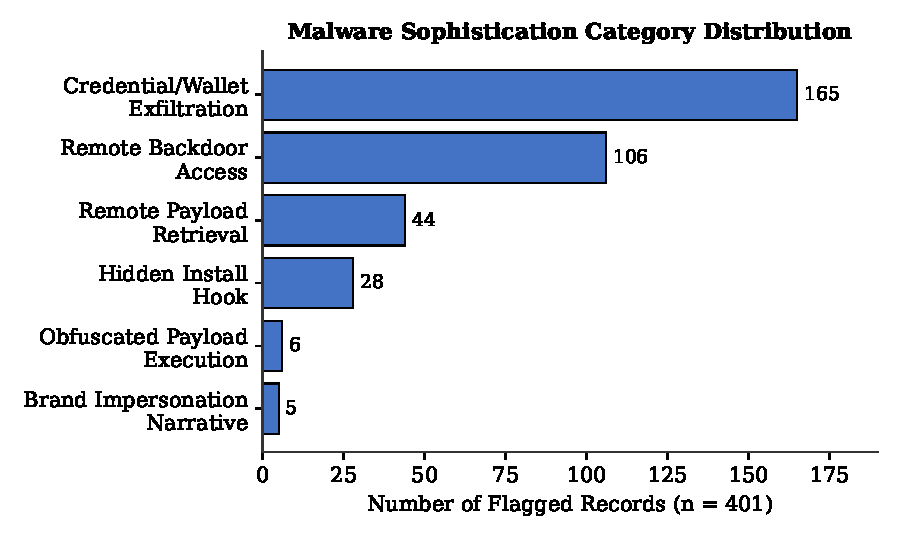
\includegraphics[width=0.48\textwidth]{prism-uploads/fig_malware_categories.pdf}
\caption{Distribution of flagged records across malware sophistication categories.}
\label{fig:categories}
\end{figure}

After the two stage campaign level collapse described in Section \ref{sec:nonindependence}, Table \ref{tab:results} reports the pooled, ecosystem stratified, and Cochran Mantel Haenszel adjusted results.

\begin{table}[h]
\centering
\caption{Final campaign level results, frozen snapshot, $n=401$ raw records collapsing to 142 independent campaigns}
\label{tab:results}
\begin{tabular}{lccc}
\toprule
Stratum & $n$ (campaigns) & Odds Ratio & $p$-value \\
\midrule
Pooled & 142 & 0.849 & 0.702 \\
npm & 42 & 1.545 & 0.530 \\
PyPI & 100 & 0.702 & 0.472 \\
CMH (ecosystem adjusted) & 142 & 0.928 & 0.848 \\
\bottomrule
\end{tabular}
\end{table}

Figure \ref{fig:odds} visualizes the final odds ratios, and Figure \ref{fig:corrections} summarizes the impact of the methodological corrections.

\begin{figure}[t]
\centering
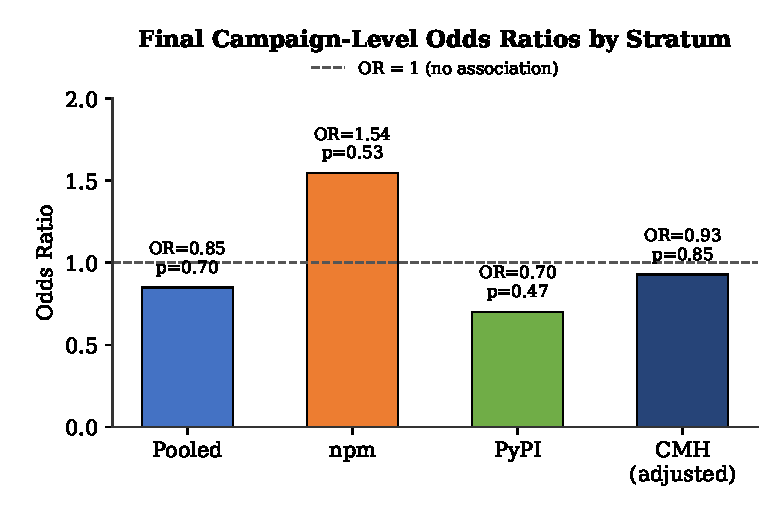
\includegraphics[width=0.48\textwidth]{prism-uploads/fig_odds_ratios.pdf}
\caption{Final campaign-level odds ratios by stratum.}
\label{fig:odds}
\end{figure}

\begin{figure}[t]
\centering
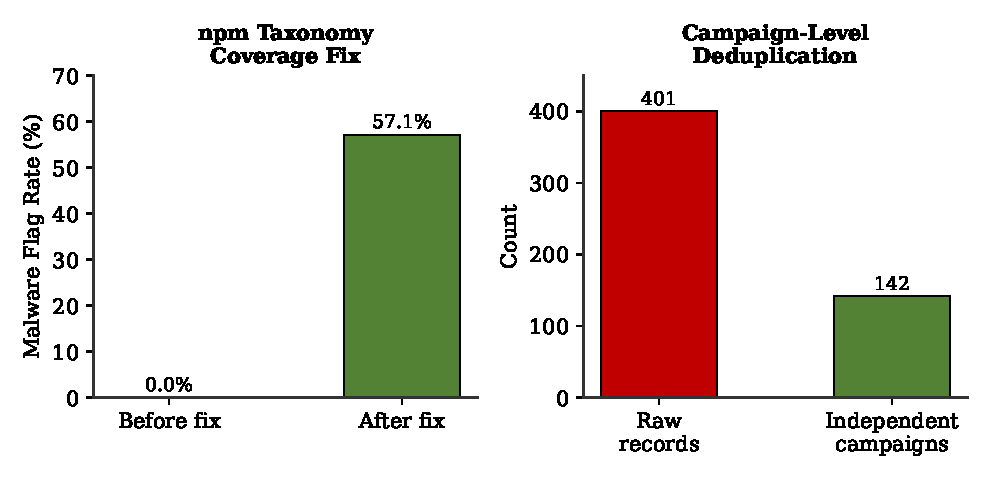
\includegraphics[width=0.48\textwidth]{prism-uploads/fig_correction_impact.pdf}
\caption{Impact of the two methodological corrections on the npm flag rate and the effective sample size.}
\label{fig:corrections}
\end{figure}

No stratum, pooled analysis, or ecosystem adjusted analysis reaches conventional statistical significance. The point estimates are directionally inconsistent across strata, with the npm stratum's odds ratio exceeding one, nominally favoring higher sophistication among grammar flagged names, while the PyPI stratum and the ecosystem adjusted estimate fall below one; given that neither individual estimate approaches significance, this directional inconsistency should be read as consistent with sampling variation around a null effect rather than as evidence of a genuine ecosystem interaction.

\section{Discussion}
\label{sec:discussion}

The corrected analysis supports no statistically significant association, in either direction, between naming grammar predictability and malware payload sophistication, pooled or after ecosystem adjustment. This finding supersedes an earlier, uncorrected reading of the same underlying research question, produced before the two corrections in Sections \ref{sec:coverage} and \ref{sec:nonindependence}, which had reported a directionally consistent, nominally significant pooled result, odds ratio approximately 0.58, $p \approx 0.046$, borderline after Cochran Mantel Haenszel adjustment, $p \approx 0.068$. That earlier reading does not survive the corrections reported in this paper; the apparent directional consistency it observed is now understood to have been partly an artifact of the npm taxonomy's near zero sensitivity described in Section \ref{sec:coverage}, which made the npm stratum trivially appear weak but same direction by construction, rather than reflecting a genuine underlying signal.

The theoretical motivation offered in Section \ref{sec:related}, drawing on the work averse attacker model \cite{allodi2021} to motivate a hypothesized negative association between naming cost and payload cost, is weakened by this null result, though not eliminated as a candidate explanation for a true effect this study is underpowered to detect. We regard it as a hypothesis worth carrying into a properly powered follow up study rather than as an explanation for an observed effect, since no effect was, in the corrected analysis, observed.

Statistical power is a central concern in interpreting this null result. The campaign level collapse described in Section \ref{sec:nonindependence}, while methodologically necessary, reduces the effective independent sample size from approximately 400 raw records to 142 independent campaigns, a reduction with direct consequences for the power of any test conducted on this corpus. A null result at $n=142$, particularly within the smaller npm stratum at $n=42$, should not be interpreted as evidence of no true effect without first establishing, via formal power analysis against the corrected campaign level sample size, what effect size the current data could plausibly detect.

\section{Threats to Validity and Limitations}
\label{sec:limitations}

Several limitations bear directly on how this result should be interpreted and reported.

First, this analysis compares grammar flagged and non flagged names within the confirmed malicious incident corpus alone, rather than against an external control sample of legitimate, non malicious packages. A 20 package control sample of popular, non flagged PyPI packages was collected and validated as a working pipeline during an earlier project phase but was never incorporated into a matched control design; this remains an open methodological decision, between incorporating the control sample into a matched comparison or explicitly justifying the within corpus comparison actually reported here, that should be resolved before this result is submitted for peer review.

Second, the malware sophistication labeler remains a heuristic candidate flagger rather than validated ground truth. No human annotated sample or inter annotator agreement study has yet been produced, a gap made more pressing by the fact that the taxonomy's pattern set changed materially in the course of producing this paper's results, as described in Section \ref{sec:coverage}.

Third, the reported association is unadjusted for covariates beyond ecosystem, specifically package age, popularity, and documentation length, each of which plausibly confounds the relationship between naming strategy and payload sophistication. A full logistic regression incorporating these controls, run on campaign level rather than raw record level units, is planned future work.

Fourth, GHSA is a live, non static data source, and record counts observed across successive pulls of the corpus varied from 395 to 401 over the project's lifetime prior to the snapshot freezing described in Section 3.1. The analysis in this paper is computed against a single frozen, checksummed snapshot specifically to eliminate this source of variation from the reported result, but any future corpus growth intended to address the power concerns in Section \ref{sec:discussion} will need to either re-freeze a new snapshot or explicitly reconcile the two.

Fifth, and more generally, the discovery of two independent, nontrivial methodological failures within a single analysis, reported transparently in this paper specifically because each generalizes beyond this study, raises the possibility that further undiscovered issues remain. We regard the discipline applied in Sections \ref{sec:coverage} and \ref{sec:nonindependence}, treating an implausible result, whether an unexpected flat zero or an implausibly large odds ratio, as a prompt for manual inspection rather than as a result to report, as the primary safeguard against this risk, and recommend the same discipline for any reader extending this corpus or this taxonomy.

\section{Future Work}
\label{sec:future}

In priority order, the following steps are identified as necessary before this line of inquiry can move from a pilot scale null result to a properly powered, publishable finding. First, a formal power analysis against the corrected campaign level sample size of 142, to establish what effect size, if any, the current data could detect, followed by corpus growth if the analysis indicates the study is underpowered at current scale. Second, resolution of the control sample gap described in Section \ref{sec:limitations}, either incorporating the existing 20 package control sample into a matched design or explicitly justifying its exclusion. Third, a full logistic regression incorporating ecosystem, package age, popularity, and documentation length as covariates, computed on campaign level units. Fourth, a human validation study of the malware sophistication labeler, including inter annotator agreement, given the taxonomy's material revision in the course of this paper. Fifth, bootstrap or exact confidence intervals on the reported odds ratios, to characterize the range of effect sizes the current data can rule out, independent of the point null hypothesis test. Sixth, a matched sample sensitivity analysis, via propensity score or exact matching, as a complement to the raw within corpus comparison reported here.

\section{Conclusion}
\label{sec:conclusion}

This paper reports a null result: no statistically significant association between predictable package naming and malware payload sophistication in a corpus of 401 confirmed malicious PyPI and npm package incidents, pooled or ecosystem adjusted, after correcting the analysis for two methodological failures, a taxonomy coverage gap specific to npm advisory language and a violation of observational independence arising from multi source and multi name campaign duplication. We present both corrections in full, alongside the final result, because the discovery pattern underlying each, stratifying by subgroup and inspecting raw matched text rather than trusting an aggregate statistic, treating an implausible result as a signal to investigate rather than to report, is reusable guidance for other security text mining pipelines built on multi source advisory corpora, independent of whether this paper's specific null result replicates at larger scale.

\begin{thebibliography}{9}

\bibitem{spracklen2024}
J.~Spracklen, R.~Wijewickrama, A.~H.~M.~N.~Sakib, A.~Maiti, B.~Viswanath, and M.~Jadliwala, ``We have a package for you! A comprehensive analysis of package hallucinations by code generating LLMs,'' \textit{arXiv preprint arXiv:2406.10279}, 2024.

\bibitem{spira2026}
A.~Spira \textit{et al.}, ``Beware of agentic botnets: Scalable untargeted promptware attacks via universal and transferable adversarial HalluSquatting,'' \textit{arXiv preprint arXiv:2607.07433}, 2026.

\bibitem{hillah2026}
L.~M.~Hillah, J.-M.~Richard, and R.~Hasnaoui, ``Bayesian-calibrated detection of hallucinated package imports in AI-assisted code,'' \textit{arXiv preprint arXiv:2606.13918}, 2026.

\bibitem{allodi2021}
L.~Allodi, F.~Massacci, and J.~Williams, ``The work-averse cyberattacker model: Theory and evidence from two million attack signatures,'' \textit{Risk Analysis}, 2021.

\bibitem{agresti}
A.~Agresti, \textit{Categorical Data Analysis}, 3rd ed. Hoboken, NJ, USA: Wiley, 2013.

\end{thebibliography}

\end{document}